\documentclass[1p]{elsarticle_modified}
%\bibliographystyle{elsarticle-num}

%\usepackage[colorlinks]{hyperref}
%\usepackage{abbrmath_seonhwa} %\Abb, \Ascr, \Acal ,\Abf, \Afrak
\usepackage{amsfonts}
\usepackage{amssymb}
\usepackage{amsmath}
\usepackage{amsthm}
\usepackage{scalefnt}
\usepackage{amsbsy}
\usepackage{kotex}
\usepackage{caption}
\usepackage{subfig}
\usepackage{color}
\usepackage{graphicx}
\usepackage{xcolor} %% white, black, red, green, blue, cyan, magenta, yellow
\usepackage{float}
\usepackage{setspace}
\usepackage{hyperref}

\usepackage{tikz}
\usetikzlibrary{arrows}

\usepackage{multirow}
\usepackage{array} % fixed length table
\usepackage{hhline}

%%%%%%%%%%%%%%%%%%%%%
\makeatletter
\renewcommand*\env@matrix[1][\arraystretch]{%
	\edef\arraystretch{#1}%
	\hskip -\arraycolsep
	\let\@ifnextchar\new@ifnextchar
	\array{*\c@MaxMatrixCols c}}
\makeatother %https://tex.stackexchange.com/questions/14071/how-can-i-increase-the-line-spacing-in-a-matrix
%%%%%%%%%%%%%%%

\usepackage[normalem]{ulem}

\newcommand{\msout}[1]{\ifmmode\text{\sout{\ensuremath{#1}}}\else\sout{#1}\fi}
%SOURCE: \msout is \stkout macro in https://tex.stackexchange.com/questions/20609/strikeout-in-math-mode

\newcommand{\cancel}[1]{
	\ifmmode
	{\color{red}\msout{#1}}
	\else
	{\color{red}\sout{#1}}
	\fi
}

\newcommand{\add}[1]{
	{\color{blue}\uwave{#1}}
}

\newcommand{\replace}[2]{
	\ifmmode
	{\color{red}\msout{#1}}{\color{blue}\uwave{#2}}
	\else
	{\color{red}\sout{#1}}{\color{blue}\uwave{#2}}
	\fi
}

\newcommand{\Sol}{\mathcal{S}} %segment
\newcommand{\D}{D} %diagram
\newcommand{\A}{\mathcal{A}} %arc


%%%%%%%%%%%%%%%%%%%%%%%%%%%%%5 test

\def\sl{\operatorname{\textup{SL}}(2,\Cbb)}
\def\psl{\operatorname{\textup{PSL}}(2,\Cbb)}
\def\quan{\mkern 1mu \triangleright \mkern 1mu}

\theoremstyle{definition}
\newtheorem{thm}{Theorem}[section]
\newtheorem{prop}[thm]{Proposition}
\newtheorem{lem}[thm]{Lemma}
\newtheorem{ques}[thm]{Question}
\newtheorem{cor}[thm]{Corollary}
\newtheorem{defn}[thm]{Definition}
\newtheorem{exam}[thm]{Example}
\newtheorem{rmk}[thm]{Remark}
\newtheorem{alg}[thm]{Algorithm}

\newcommand{\I}{\sqrt{-1}}
\begin{document}

%\begin{frontmatter}
%
%\title{Boundary parabolic representations of knots up to 8 crossings}
%
%%% Group authors per affiliation:
%\author{Yunhi Cho} 
%\address{Department of Mathematics, University of Seoul, Seoul, Korea}
%\ead{yhcho@uos.ac.kr}
%
%
%\author{Seonhwa Kim} %\fnref{s_kim}}
%\address{Center for Geometry and Physics, Institute for Basic Science, Pohang, 37673, Korea}
%\ead{ryeona17@ibs.re.kr}
%
%\author{Hyuk Kim}
%\address{Department of Mathematical Sciences, Seoul National University, Seoul 08826, Korea}
%\ead{hyukkim@snu.ac.kr}
%
%\author{Seokbeom Yoon}
%\address{Department of Mathematical Sciences, Seoul National University, Seoul, 08826,  Korea}
%\ead{sbyoon15@snu.ac.kr}
%
%\begin{abstract}
%We find all boundary parabolic representation of knots up to 8 crossings.
%
%\end{abstract}
%\begin{keyword}
%    \MSC[2010] 57M25 
%\end{keyword}
%
%\end{frontmatter}

%\linenumbers
%\tableofcontents
%
\newcommand\colored[1]{\textcolor{white}{\rule[-0.35ex]{0.8em}{1.4ex}}\kern-0.8em\color{red} #1}%
%\newcommand\colored[1]{\textcolor{white}{ #1}\kern-2.17ex	\textcolor{white}{ #1}\kern-1.81ex	\textcolor{white}{ #1}\kern-2.15ex\color{red}#1	}

{\Large $\underline{12n_{0832}~(K12n_{0832})}$}

\setlength{\tabcolsep}{10pt}
\renewcommand{\arraystretch}{1.6}
\vspace{1cm}\begin{tabular}{m{100pt}>{\centering\arraybackslash}m{274pt}}
\multirow{5}{120pt}{
	\centering
	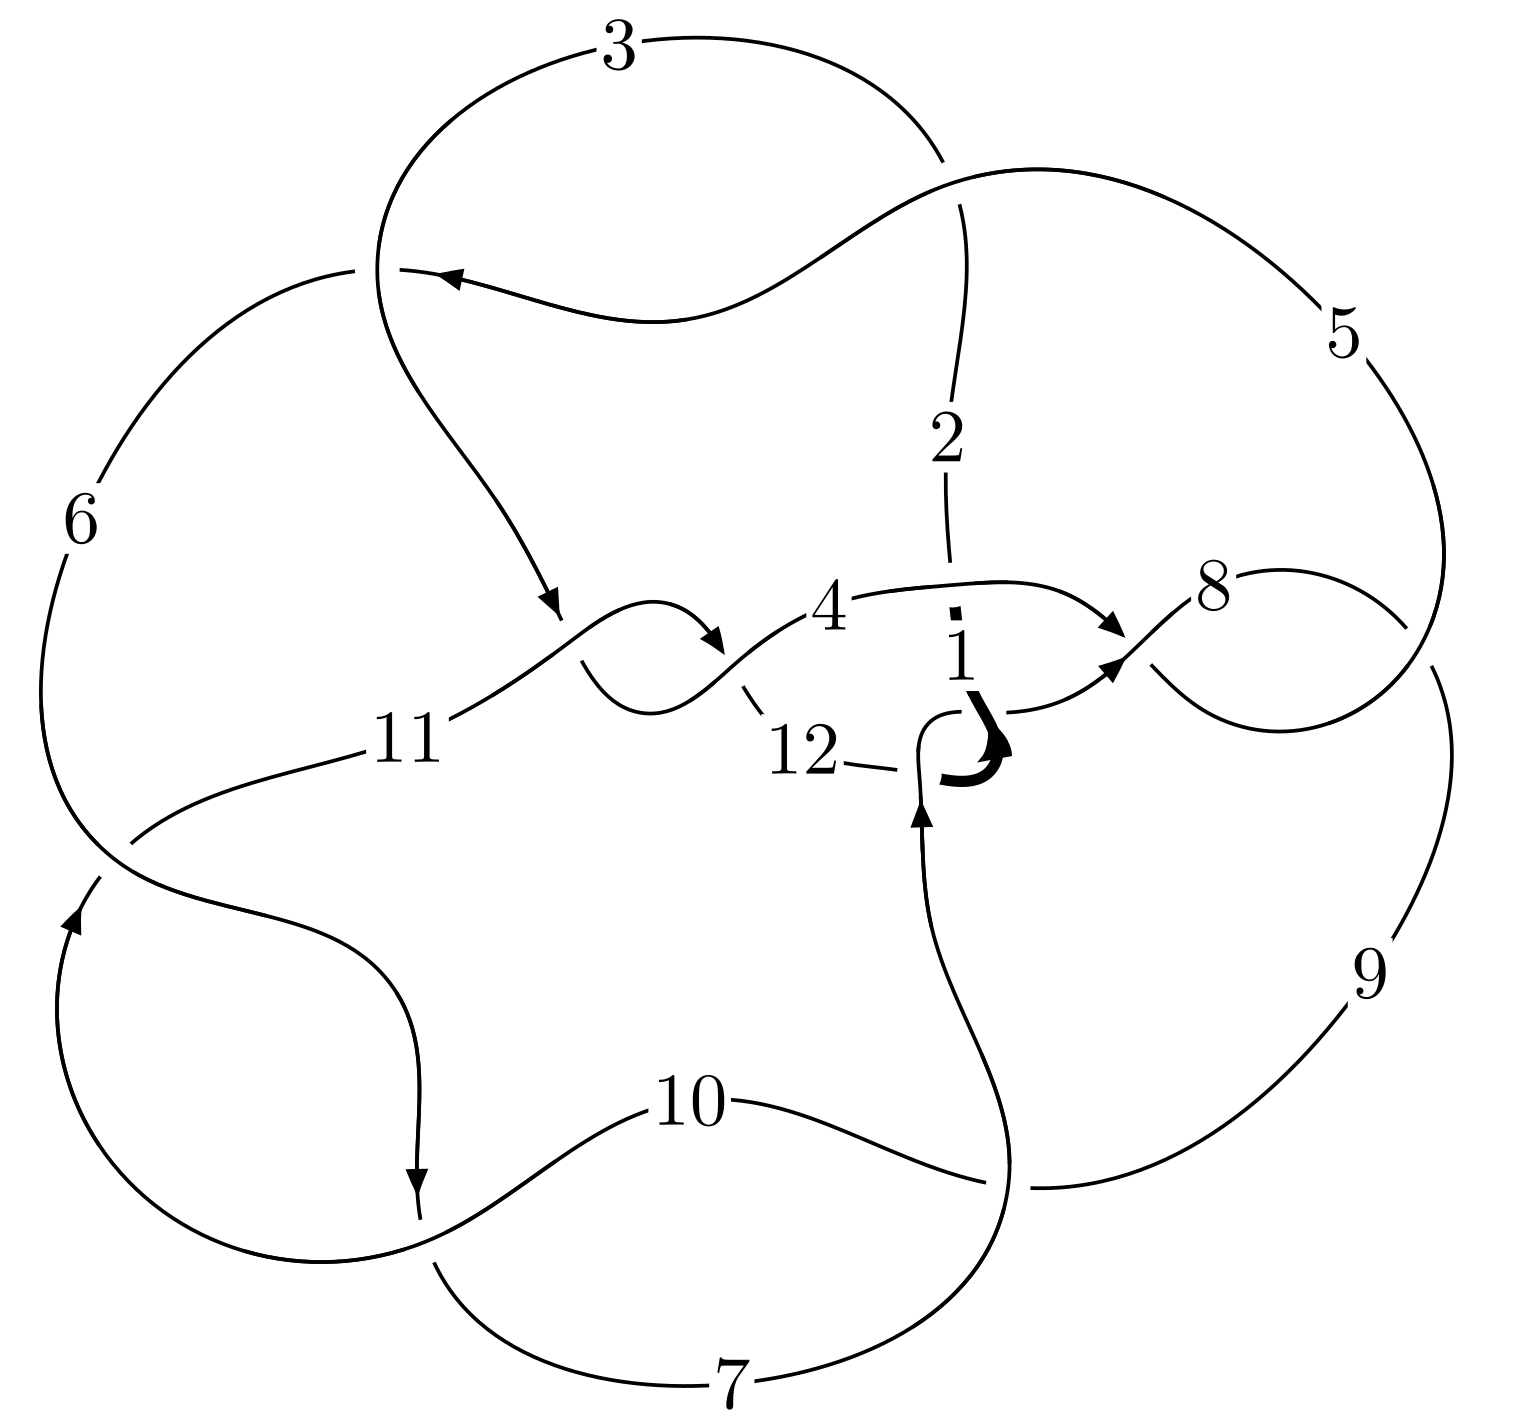
\includegraphics[width=112pt]{../../../GIT/diagram.site/Diagrams/png/2921_12n_0832.png}\\
\ \ \ A knot diagram\footnotemark}&
\allowdisplaybreaks
\textbf{Linearized knot diagam} \\
\cline{2-2}
 &
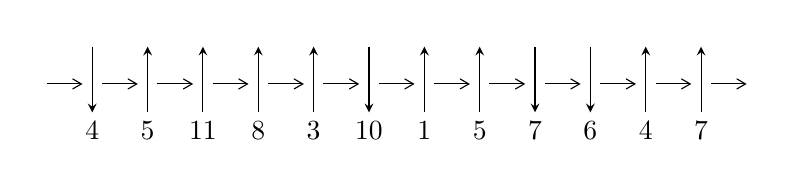
\begin{tikzpicture}[x=20pt, y=17pt]
	% nodes
	\node (C0) at (0, 0) {};
	\node (C1) at (1, 0) {};
	\node (C1U) at (1, +1) {};
	\node (C1D) at (1, -1) {4};

	\node (C2) at (2, 0) {};
	\node (C2U) at (2, +1) {};
	\node (C2D) at (2, -1) {5};

	\node (C3) at (3, 0) {};
	\node (C3U) at (3, +1) {};
	\node (C3D) at (3, -1) {11};

	\node (C4) at (4, 0) {};
	\node (C4U) at (4, +1) {};
	\node (C4D) at (4, -1) {8};

	\node (C5) at (5, 0) {};
	\node (C5U) at (5, +1) {};
	\node (C5D) at (5, -1) {3};

	\node (C6) at (6, 0) {};
	\node (C6U) at (6, +1) {};
	\node (C6D) at (6, -1) {10};

	\node (C7) at (7, 0) {};
	\node (C7U) at (7, +1) {};
	\node (C7D) at (7, -1) {1};

	\node (C8) at (8, 0) {};
	\node (C8U) at (8, +1) {};
	\node (C8D) at (8, -1) {5};

	\node (C9) at (9, 0) {};
	\node (C9U) at (9, +1) {};
	\node (C9D) at (9, -1) {7};

	\node (C10) at (10, 0) {};
	\node (C10U) at (10, +1) {};
	\node (C10D) at (10, -1) {6};

	\node (C11) at (11, 0) {};
	\node (C11U) at (11, +1) {};
	\node (C11D) at (11, -1) {4};

	\node (C12) at (12, 0) {};
	\node (C12U) at (12, +1) {};
	\node (C12D) at (12, -1) {7};
	\node (C13) at (13, 0) {};

	% arrows
	\draw[->,>={angle 60}]
	(C0) edge (C1) (C1) edge (C2) (C2) edge (C3) (C3) edge (C4) (C4) edge (C5) (C5) edge (C6) (C6) edge (C7) (C7) edge (C8) (C8) edge (C9) (C9) edge (C10) (C10) edge (C11) (C11) edge (C12) (C12) edge (C13) ;	\draw[->,>=stealth]
	(C1U) edge (C1D) (C2D) edge (C2U) (C3D) edge (C3U) (C4D) edge (C4U) (C5D) edge (C5U) (C6U) edge (C6D) (C7D) edge (C7U) (C8D) edge (C8U) (C9U) edge (C9D) (C10U) edge (C10D) (C11D) edge (C11U) (C12D) edge (C12U) ;
	\end{tikzpicture} \\
\hhline{~~} \\& 
\textbf{Solving Sequence} \\ \cline{2-2} 
 &
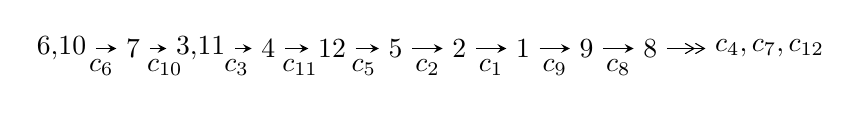
\begin{tikzpicture}[x=23pt, y=7pt]
	% node
	\node (A0) at (-1/8, 0) {6,10};
	\node (A1) at (1, 0) {7};
	\node (A2) at (33/16, 0) {3,11};
	\node (A3) at (25/8, 0) {4};
	\node (A4) at (33/8, 0) {12};
	\node (A5) at (41/8, 0) {5};
	\node (A6) at (49/8, 0) {2};
	\node (A7) at (57/8, 0) {1};
	\node (A8) at (65/8, 0) {9};
	\node (A9) at (73/8, 0) {8};
	\node (C1) at (1/2, -1) {$c_{6}$};
	\node (C2) at (3/2, -1) {$c_{10}$};
	\node (C3) at (21/8, -1) {$c_{3}$};
	\node (C4) at (29/8, -1) {$c_{11}$};
	\node (C5) at (37/8, -1) {$c_{5}$};
	\node (C6) at (45/8, -1) {$c_{2}$};
	\node (C7) at (53/8, -1) {$c_{1}$};
	\node (C8) at (61/8, -1) {$c_{9}$};
	\node (C9) at (69/8, -1) {$c_{8}$};
	\node (A10) at (11, 0) {$c_{4},c_{7},c_{12}$};

	% edge
	\draw[->,>=stealth]	
	(A0) edge (A1) (A1) edge (A2) (A2) edge (A3) (A3) edge (A4) (A4) edge (A5) (A5) edge (A6) (A6) edge (A7) (A7) edge (A8) (A8) edge (A9) ;
	\draw[->>,>={angle 60}]	
	(A9) edge (A10);
\end{tikzpicture} \\ 

\end{tabular} \\

\footnotetext{
The image of knot diagram is generated by the software ``\textbf{Draw programme}" developed by Andrew Bartholomew(\url{http://www.layer8.co.uk/maths/draw/index.htm\#Running-draw}), where we modified some parts for our purpose(\url{https://github.com/CATsTAILs/LinksPainter}).
}\phantom \\ \newline 
\centering \textbf{Ideals for irreducible components\footnotemark of $X_{\text{par}}$} 
 
\begin{align*}
I^u_{1}&=\langle 
755 u^{20}-5418 u^{19}+\cdots+1124 b+9500,\;865 u^{20}-6654 u^{19}+\cdots+2248 a-4904,\\
\phantom{I^u_{1}}&\phantom{= \langle  }u^{21}-8 u^{20}+\cdots+84 u-8\rangle \\
I^u_{2}&=\langle 
u^{25} a+113 u^{25}+\cdots- a-113,\;- u^{25} a+59 u^{25}+\cdots+35 a-380,\;u^{26}+3 u^{25}+\cdots-10 u-1\rangle \\
I^u_{3}&=\langle 
u^{10}- u^9+6 u^8-5 u^7+13 u^6-8 u^5+13 u^4-4 u^3+6 u^2+b+1,\\
\phantom{I^u_{3}}&\phantom{= \langle  }u^9+5 u^7+8 u^5+u^4+5 u^3+4 u^2+a+2 u+3,\\
\phantom{I^u_{3}}&\phantom{= \langle  }u^{11}- u^{10}+7 u^9-6 u^8+18 u^7-13 u^6+22 u^5-12 u^4+14 u^3-4 u^2+4 u-1\rangle \\
I^u_{4}&=\langle 
- u^4 a+u^3 a- u^4-4 u^2 a+u^3+4 a u-4 u^2+5 b- a+4 u-6,\;u^4 a+3 u^2 a- u^3+a^2+3 a- u-1,\\
\phantom{I^u_{4}}&\phantom{= \langle  }u^5+3 u^3+2 u+1\rangle \\
\\
\end{align*}
\raggedright * 4 irreducible components of $\dim_{\mathbb{C}}=0$, with total 94 representations.\\
\footnotetext{All coefficients of polynomials are rational numbers. But the coefficients are sometimes approximated in decimal forms when there is not enough margin.}
\newpage
\renewcommand{\arraystretch}{1}
\centering \section*{I. $I^u_{1}= \langle 755 u^{20}-5418 u^{19}+\cdots+1124 b+9500,\;865 u^{20}-6654 u^{19}+\cdots+2248 a-4904,\;u^{21}-8 u^{20}+\cdots+84 u-8 \rangle$}
\flushleft \textbf{(i) Arc colorings}\\
\begin{tabular}{m{7pt} m{180pt} m{7pt} m{180pt} }
\flushright $a_{6}=$&$\begin{pmatrix}1\\0\end{pmatrix}$ \\
\flushright $a_{10}=$&$\begin{pmatrix}0\\u\end{pmatrix}$ \\
\flushright $a_{7}=$&$\begin{pmatrix}1\\u^2\end{pmatrix}$ \\
\flushright $a_{3}=$&$\begin{pmatrix}-0.384786 u^{20}+2.95996 u^{19}+\cdots+3.87811 u+2.18149\\-0.671708 u^{20}+4.82028 u^{19}+\cdots+82.4751 u-8.45196\end{pmatrix}$ \\
\flushright $a_{11}=$&$\begin{pmatrix}- u\\u\end{pmatrix}$ \\
\flushright $a_{4}=$&$\begin{pmatrix}-0.938167 u^{20}+6.46886 u^{19}+\cdots+51.8496 u-3.19217\\-0.118327 u^{20}+1.31139 u^{19}+\cdots+34.5036 u-3.07829\end{pmatrix}$ \\
\flushright $a_{12}=$&$\begin{pmatrix}-1.46486 u^{20}+10.4733 u^{19}+\cdots+114.085 u-10.8790\\-0.601423 u^{20}+4.76690 u^{19}+\cdots+65.6459 u-6.20996\end{pmatrix}$ \\
\flushright $a_{5}=$&$\begin{pmatrix}-0.776246 u^{20}+5.60854 u^{19}+\cdots+23.2527 u+0.441281\\-1.29004 u^{20}+9.63167 u^{19}+\cdots+156.479 u-16.5302\end{pmatrix}$ \\
\flushright $a_{2}=$&$\begin{pmatrix}0.978203 u^{20}-6.60053 u^{19}+\cdots-67.8283 u+8.22242\\0.298043 u^{20}-2.75801 u^{19}+\cdots-46.1744 u+4.83630\end{pmatrix}$ \\
\flushright $a_{1}=$&$\begin{pmatrix}-1.14279 u^{20}+8.33630 u^{19}+\cdots+86.8238 u-7.12456\\-0.241993 u^{20}+1.87367 u^{19}+\cdots+31.3043 u-2.69395\end{pmatrix}$ \\
\flushright $a_{9}=$&$\begin{pmatrix}u\\u^3+u\end{pmatrix}$ \\
\flushright $a_{8}=$&$\begin{pmatrix}-0.424822 u^{20}+3.09164 u^{19}+\cdots+19.8568 u-2.84875\\1.07206 u^{20}-7.63701 u^{19}+\cdots-71.7616 u+7.75445\end{pmatrix}$\\&\end{tabular}
\flushleft \textbf{(ii) Obstruction class $= -1$}\\~\\
\flushleft \textbf{(iii) Cusp Shapes $= \frac{797}{281} u^{20}-\frac{5987}{281} u^{19}+\cdots-\frac{114148}{281} u+\frac{15414}{281}$}\\~\\
\newpage\renewcommand{\arraystretch}{1}
\flushleft \textbf{(iv) u-Polynomials at the component}\newline \\
\begin{tabular}{m{50pt}|m{274pt}}
Crossings & \hspace{64pt}u-Polynomials at each crossing \\
\hline $$\begin{aligned}c_{1}\end{aligned}$$&$\begin{aligned}
&u^{21}-20 u^{20}+\cdots+1600 u-128
\end{aligned}$\\
\hline $$\begin{aligned}c_{2},c_{3},c_{5}\\c_{11}\end{aligned}$$&$\begin{aligned}
&u^{21}-8 u^{19}+\cdots-3 u-1
\end{aligned}$\\
\hline $$\begin{aligned}c_{4},c_{7},c_{8}\\c_{12}\end{aligned}$$&$\begin{aligned}
&u^{21}-5 u^{19}+\cdots+2 u-1
\end{aligned}$\\
\hline $$\begin{aligned}c_{6},c_{9},c_{10}\end{aligned}$$&$\begin{aligned}
&u^{21}-8 u^{20}+\cdots+84 u-8
\end{aligned}$\\
\hline
\end{tabular}\\~\\
\newpage\renewcommand{\arraystretch}{1}
\flushleft \textbf{(v) Riley Polynomials at the component}\newline \\
\begin{tabular}{m{50pt}|m{274pt}}
Crossings & \hspace{64pt}Riley Polynomials at each crossing \\
\hline $$\begin{aligned}c_{1}\end{aligned}$$&$\begin{aligned}
&y^{21}+6 y^{20}+\cdots-692224 y-16384
\end{aligned}$\\
\hline $$\begin{aligned}c_{2},c_{3},c_{5}\\c_{11}\end{aligned}$$&$\begin{aligned}
&y^{21}-16 y^{20}+\cdots+25 y-1
\end{aligned}$\\
\hline $$\begin{aligned}c_{4},c_{7},c_{8}\\c_{12}\end{aligned}$$&$\begin{aligned}
&y^{21}-10 y^{20}+\cdots+12 y-1
\end{aligned}$\\
\hline $$\begin{aligned}c_{6},c_{9},c_{10}\end{aligned}$$&$\begin{aligned}
&y^{21}+20 y^{20}+\cdots+528 y-64
\end{aligned}$\\
\hline
\end{tabular}\\~\\
\newpage\flushleft \textbf{(vi) Complex Volumes and Cusp Shapes}
$$\begin{array}{c|c|c}  
\text{Solutions to }I^u_{1}& \I (\text{vol} + \sqrt{-1}CS) & \text{Cusp shape}\\
 \hline 
\begin{aligned}
u &= -0.430675 + 0.863692 I \\
a &= \phantom{-}0.474474 + 0.031759 I \\
b &= -0.241235 + 0.131245 I\end{aligned}
 & \phantom{-}0.31209 + 1.75113 I & \phantom{-}3.06893 - 1.22304 I \\ \hline\begin{aligned}
u &= -0.430675 - 0.863692 I \\
a &= \phantom{-}0.474474 - 0.031759 I \\
b &= -0.241235 - 0.131245 I\end{aligned}
 & \phantom{-}0.31209 - 1.75113 I & \phantom{-}3.06893 + 1.22304 I \\ \hline\begin{aligned}
u &= \phantom{-}0.941579 + 0.500830 I \\
a &= \phantom{-}0.468449 + 0.441296 I \\
b &= -1.230110 + 0.582897 I\end{aligned}
 & \phantom{-}2.10752 - 11.16100 I & \phantom{-}8.47490 + 8.35858 I \\ \hline\begin{aligned}
u &= \phantom{-}0.941579 - 0.500830 I \\
a &= \phantom{-}0.468449 - 0.441296 I \\
b &= -1.230110 - 0.582897 I\end{aligned}
 & \phantom{-}2.10752 + 11.16100 I & \phantom{-}8.47490 - 8.35858 I \\ \hline\begin{aligned}
u &= \phantom{-}0.864822 + 0.780507 I \\
a &= \phantom{-}0.228758 + 0.686980 I \\
b &= -1.034020 - 0.254427 I\end{aligned}
 & \phantom{-}2.88881 + 5.10968 I & \phantom{-}10.51418 - 4.53183 I \\ \hline\begin{aligned}
u &= \phantom{-}0.864822 - 0.780507 I \\
a &= \phantom{-}0.228758 - 0.686980 I \\
b &= -1.034020 + 0.254427 I\end{aligned}
 & \phantom{-}2.88881 - 5.10968 I & \phantom{-}10.51418 + 4.53183 I \\ \hline\begin{aligned}
u &= \phantom{-}0.784060 + 0.089570 I \\
a &= \phantom{-}0.148949 - 0.280369 I \\
b &= \phantom{-}0.899061 - 0.583293 I\end{aligned}
 & -0.161111 + 0.298509 I & \phantom{-}5.89200 - 0.80081 I \\ \hline\begin{aligned}
u &= \phantom{-}0.784060 - 0.089570 I \\
a &= \phantom{-}0.148949 + 0.280369 I \\
b &= \phantom{-}0.899061 + 0.583293 I\end{aligned}
 & -0.161111 - 0.298509 I & \phantom{-}5.89200 + 0.80081 I \\ \hline\begin{aligned}
u &= \phantom{-}0.337572 + 0.642009 I \\
a &= -1.027230 - 0.769285 I \\
b &= \phantom{-}0.807982 - 0.604519 I\end{aligned}
 & \phantom{-}2.55000 - 2.18542 I & \phantom{-}13.17858 + 4.25561 I \\ \hline\begin{aligned}
u &= \phantom{-}0.337572 - 0.642009 I \\
a &= -1.027230 + 0.769285 I \\
b &= \phantom{-}0.807982 + 0.604519 I\end{aligned}
 & \phantom{-}2.55000 + 2.18542 I & \phantom{-}13.17858 - 4.25561 I\\
 \hline 
 \end{array}$$\newpage$$\begin{array}{c|c|c}  
\text{Solutions to }I^u_{1}& \I (\text{vol} + \sqrt{-1}CS) & \text{Cusp shape}\\
 \hline 
\begin{aligned}
u &= \phantom{-}0.445135 + 1.219610 I \\
a &= -0.175359 - 0.810246 I \\
b &= \phantom{-}0.671583 + 0.440706 I\end{aligned}
 & \phantom{-}3.28725 - 4.77138 I & \phantom{-}12.62050 + 2.51819 I \\ \hline\begin{aligned}
u &= \phantom{-}0.445135 - 1.219610 I \\
a &= -0.175359 + 0.810246 I \\
b &= \phantom{-}0.671583 - 0.440706 I\end{aligned}
 & \phantom{-}3.28725 + 4.77138 I & \phantom{-}12.62050 - 2.51819 I \\ \hline\begin{aligned}
u &= \phantom{-}0.274538 + 1.362470 I \\
a &= -1.61794 - 0.34738 I \\
b &= \phantom{-}1.32395 - 0.68359 I\end{aligned}
 & \phantom{-}4.45013 - 3.41075 I & \phantom{-}7.62872 + 0.78780 I \\ \hline\begin{aligned}
u &= \phantom{-}0.274538 - 1.362470 I \\
a &= -1.61794 + 0.34738 I \\
b &= \phantom{-}1.32395 + 0.68359 I\end{aligned}
 & \phantom{-}4.45013 + 3.41075 I & \phantom{-}7.62872 - 0.78780 I \\ \hline\begin{aligned}
u &= \phantom{-}0.09790 + 1.57918 I \\
a &= -1.59282 + 0.10699 I \\
b &= \phantom{-}1.107320 - 0.838285 I\end{aligned}
 & \phantom{-}10.08840 - 3.80196 I & \phantom{-}14.3317 + 1.4217 I \\ \hline\begin{aligned}
u &= \phantom{-}0.09790 - 1.57918 I \\
a &= -1.59282 - 0.10699 I \\
b &= \phantom{-}1.107320 + 0.838285 I\end{aligned}
 & \phantom{-}10.08840 + 3.80196 I & \phantom{-}14.3317 - 1.4217 I \\ \hline\begin{aligned}
u &= \phantom{-}0.34514 + 1.54955 I \\
a &= \phantom{-}1.75952 + 0.28354 I \\
b &= -1.50761 + 0.74551 I\end{aligned}
 & \phantom{-}8.7389 - 15.8550 I & \phantom{-}11.09832 + 8.19798 I \\ \hline\begin{aligned}
u &= \phantom{-}0.34514 - 1.54955 I \\
a &= \phantom{-}1.75952 - 0.28354 I \\
b &= -1.50761 - 0.74551 I\end{aligned}
 & \phantom{-}8.7389 + 15.8550 I & \phantom{-}11.09832 - 8.19798 I \\ \hline\begin{aligned}
u &= \phantom{-}0.19250 + 1.66330 I \\
a &= \phantom{-}1.163750 + 0.386362 I \\
b &= -1.076850 + 0.271112 I\end{aligned}
 & \phantom{-}11.34600 + 1.18083 I & \phantom{-}12.33791 - 3.38306 I \\ \hline\begin{aligned}
u &= \phantom{-}0.19250 - 1.66330 I \\
a &= \phantom{-}1.163750 - 0.386362 I \\
b &= -1.076850 - 0.271112 I\end{aligned}
 & \phantom{-}11.34600 - 1.18083 I & \phantom{-}12.33791 + 3.38306 I\\
 \hline 
 \end{array}$$\newpage$$\begin{array}{c|c|c}  
\text{Solutions to }I^u_{1}& \I (\text{vol} + \sqrt{-1}CS) & \text{Cusp shape}\\
 \hline 
\begin{aligned}
u &= \phantom{-}0.294851\phantom{ +0.000000I} \\
a &= \phantom{-}1.33890\phantom{ +0.000000I} \\
b &= \phantom{-}0.559847\phantom{ +0.000000I}\end{aligned}
 & \phantom{-}0.900446\phantom{ +0.000000I} & \phantom{-}10.7090\phantom{ +0.000000I}\\
 \hline 
 \end{array}$$\newpage\newpage\renewcommand{\arraystretch}{1}
\centering \section*{II. $I^u_{2}= \langle u^{25} a+113 u^{25}+\cdots- a-113,\;- u^{25} a+59 u^{25}+\cdots+35 a-380,\;u^{26}+3 u^{25}+\cdots-10 u-1 \rangle$}
\flushleft \textbf{(i) Arc colorings}\\
\begin{tabular}{m{7pt} m{180pt} m{7pt} m{180pt} }
\flushright $a_{6}=$&$\begin{pmatrix}1\\0\end{pmatrix}$ \\
\flushright $a_{10}=$&$\begin{pmatrix}0\\u\end{pmatrix}$ \\
\flushright $a_{7}=$&$\begin{pmatrix}1\\u^2\end{pmatrix}$ \\
\flushright $a_{3}=$&$\begin{pmatrix}a\\-0.00204918 a u^{25}-0.231557 u^{25}+\cdots+0.00204918 a+0.231557\end{pmatrix}$ \\
\flushright $a_{11}=$&$\begin{pmatrix}- u\\u\end{pmatrix}$ \\
\flushright $a_{4}=$&$\begin{pmatrix}-0.00204918 a u^{25}+1.01844 u^{25}+\cdots+1.00205 a-0.0184426\\-\frac{5}{4} u^{25}-\frac{13}{4} u^{24}+\cdots-\frac{25}{4} u+\frac{1}{4}\end{pmatrix}$ \\
\flushright $a_{12}=$&$\begin{pmatrix}0.786885 a u^{25}+3.41803 u^{25}+\cdots+0.213115 a-17.9180\\-1.01844 a u^{25}-0.334016 u^{25}+\cdots+0.0184426 a-2.66598\end{pmatrix}$ \\
\flushright $a_{5}=$&$\begin{pmatrix}-0.0184426 a u^{25}-2.08402 u^{25}+\cdots-0.231557 a+17.8340\\0.0184426 a u^{25}-1.66598 u^{25}+\cdots+0.231557 a+3.41598\end{pmatrix}$ \\
\flushright $a_{2}=$&$\begin{pmatrix}1.08607 a u^{25}+3.60041 u^{25}+\cdots-2.08607 a-18.8504\\-0.573770 a u^{25}+0.913934 u^{25}+\cdots-1.17623 a-8.41393\end{pmatrix}$ \\
\flushright $a_{1}=$&$\begin{pmatrix}0.231557 a u^{25}+2.91598 u^{25}+\cdots+0.768443 a-19.1660\\-0.323770 a u^{25}+1.16393 u^{25}+\cdots-0.176230 a-3.66393\end{pmatrix}$ \\
\flushright $a_{9}=$&$\begin{pmatrix}u\\u^3+u\end{pmatrix}$ \\
\flushright $a_{8}=$&$\begin{pmatrix}u^{25} a-\frac{1}{4} u^{25}+\cdots-\frac{11}{4} a+\frac{35}{4}\\-0.512295 a u^{25}-0.764344 u^{25}+\cdots+1.26230 a+5.76434\end{pmatrix}$\\&\end{tabular}
\flushleft \textbf{(ii) Obstruction class $= -1$}\\~\\
\flushleft \textbf{(iii) Cusp Shapes $= -6 u^{25}-16 u^{24}-101 u^{23}-221 u^{22}-726 u^{21}-1318 u^{20}-2920 u^{19}-4393 u^{18}-7154 u^{17}-8772 u^{16}-10705 u^{15}-10189 u^{14}-8827 u^{13}-5415 u^{12}-2068 u^{11}+1201 u^{10}+2439 u^9+3056 u^8+1615 u^7+1083 u^6-79 u^5-164 u^4-80 u^3-87 u^2+98 u+43$}\\~\\
\newpage\renewcommand{\arraystretch}{1}
\flushleft \textbf{(iv) u-Polynomials at the component}\newline \\
\begin{tabular}{m{50pt}|m{274pt}}
Crossings & \hspace{64pt}u-Polynomials at each crossing \\
\hline $$\begin{aligned}c_{1}\end{aligned}$$&$\begin{aligned}
&(u^{26}+4 u^{25}+\cdots-14 u-1)^{2}
\end{aligned}$\\
\hline $$\begin{aligned}c_{2},c_{3},c_{5}\\c_{11}\end{aligned}$$&$\begin{aligned}
&u^{52}-16 u^{50}+\cdots-18950 u-3929
\end{aligned}$\\
\hline $$\begin{aligned}c_{4},c_{7},c_{8}\\c_{12}\end{aligned}$$&$\begin{aligned}
&u^{52}- u^{51}+\cdots-116 u-173
\end{aligned}$\\
\hline $$\begin{aligned}c_{6},c_{9},c_{10}\end{aligned}$$&$\begin{aligned}
&(u^{26}+3 u^{25}+\cdots-10 u-1)^{2}
\end{aligned}$\\
\hline
\end{tabular}\\~\\
\newpage\renewcommand{\arraystretch}{1}
\flushleft \textbf{(v) Riley Polynomials at the component}\newline \\
\begin{tabular}{m{50pt}|m{274pt}}
Crossings & \hspace{64pt}Riley Polynomials at each crossing \\
\hline $$\begin{aligned}c_{1}\end{aligned}$$&$\begin{aligned}
&(y^{26}-10 y^{25}+\cdots-44 y+1)^{2}
\end{aligned}$\\
\hline $$\begin{aligned}c_{2},c_{3},c_{5}\\c_{11}\end{aligned}$$&$\begin{aligned}
&y^{52}-32 y^{51}+\cdots-267831830 y+15437041
\end{aligned}$\\
\hline $$\begin{aligned}c_{4},c_{7},c_{8}\\c_{12}\end{aligned}$$&$\begin{aligned}
&y^{52}-25 y^{51}+\cdots-356688 y+29929
\end{aligned}$\\
\hline $$\begin{aligned}c_{6},c_{9},c_{10}\end{aligned}$$&$\begin{aligned}
&(y^{26}+27 y^{25}+\cdots-64 y+1)^{2}
\end{aligned}$\\
\hline
\end{tabular}\\~\\
\newpage\flushleft \textbf{(vi) Complex Volumes and Cusp Shapes}
$$\begin{array}{c|c|c}  
\text{Solutions to }I^u_{2}& \I (\text{vol} + \sqrt{-1}CS) & \text{Cusp shape}\\
 \hline 
\begin{aligned}
u &= -0.936700 + 0.371884 I \\
a &= \phantom{-}0.462570 - 0.350885 I \\
b &= -1.195860 - 0.440014 I\end{aligned}
 & -0.05500 + 4.49672 I & \phantom{-}6.90644 - 6.32358 I \\ \hline\begin{aligned}
u &= -0.936700 + 0.371884 I \\
a &= -0.039258 + 0.375495 I \\
b &= \phantom{-}0.980992 + 0.468137 I\end{aligned}
 & -0.05500 + 4.49672 I & \phantom{-}6.90644 - 6.32358 I \\ \hline\begin{aligned}
u &= -0.936700 - 0.371884 I \\
a &= \phantom{-}0.462570 + 0.350885 I \\
b &= -1.195860 + 0.440014 I\end{aligned}
 & -0.05500 - 4.49672 I & \phantom{-}6.90644 + 6.32358 I \\ \hline\begin{aligned}
u &= -0.936700 - 0.371884 I \\
a &= -0.039258 - 0.375495 I \\
b &= \phantom{-}0.980992 - 0.468137 I\end{aligned}
 & -0.05500 - 4.49672 I & \phantom{-}6.90644 + 6.32358 I \\ \hline\begin{aligned}
u &= \phantom{-}0.161010 + 0.937138 I \\
a &= -0.372337 - 0.320316 I \\
b &= \phantom{-}0.594088 + 0.976193 I\end{aligned}
 & \phantom{-}1.50012 + 2.81558 I & \phantom{-}10.54904 - 1.62602 I \\ \hline\begin{aligned}
u &= \phantom{-}0.161010 + 0.937138 I \\
a &= \phantom{-}1.69655 - 0.75534 I \\
b &= -0.578944 + 0.313413 I\end{aligned}
 & \phantom{-}1.50012 + 2.81558 I & \phantom{-}10.54904 - 1.62602 I \\ \hline\begin{aligned}
u &= \phantom{-}0.161010 - 0.937138 I \\
a &= -0.372337 + 0.320316 I \\
b &= \phantom{-}0.594088 - 0.976193 I\end{aligned}
 & \phantom{-}1.50012 - 2.81558 I & \phantom{-}10.54904 + 1.62602 I \\ \hline\begin{aligned}
u &= \phantom{-}0.161010 - 0.937138 I \\
a &= \phantom{-}1.69655 + 0.75534 I \\
b &= -0.578944 - 0.313413 I\end{aligned}
 & \phantom{-}1.50012 - 2.81558 I & \phantom{-}10.54904 + 1.62602 I \\ \hline\begin{aligned}
u &= -0.708992 + 0.951444 I \\
a &= \phantom{-}0.651485 - 0.808528 I \\
b &= -1.011240 + 0.204754 I\end{aligned}
 & \phantom{-}1.64103 + 1.22347 I & \phantom{-}13.51964 + 0.98097 I \\ \hline\begin{aligned}
u &= -0.708992 + 0.951444 I \\
a &= -0.181917 + 0.494490 I \\
b &= \phantom{-}0.829524 + 0.085781 I\end{aligned}
 & \phantom{-}1.64103 + 1.22347 I & \phantom{-}13.51964 + 0.98097 I\\
 \hline 
 \end{array}$$\newpage$$\begin{array}{c|c|c}  
\text{Solutions to }I^u_{2}& \I (\text{vol} + \sqrt{-1}CS) & \text{Cusp shape}\\
 \hline 
\begin{aligned}
u &= -0.708992 - 0.951444 I \\
a &= \phantom{-}0.651485 + 0.808528 I \\
b &= -1.011240 - 0.204754 I\end{aligned}
 & \phantom{-}1.64103 - 1.22347 I & \phantom{-}13.51964 - 0.98097 I \\ \hline\begin{aligned}
u &= -0.708992 - 0.951444 I \\
a &= -0.181917 - 0.494490 I \\
b &= \phantom{-}0.829524 - 0.085781 I\end{aligned}
 & \phantom{-}1.64103 - 1.22347 I & \phantom{-}13.51964 - 0.98097 I \\ \hline\begin{aligned}
u &= -0.182776 + 1.209640 I \\
a &= -0.090918 - 0.481727 I \\
b &= \phantom{-}0.060610 + 1.140650 I\end{aligned}
 & \phantom{-}0.96206 + 2.92695 I & \phantom{-}6.81519 - 4.13402 I \\ \hline\begin{aligned}
u &= -0.182776 + 1.209640 I \\
a &= \phantom{-}1.70603 - 0.03119 I \\
b &= -0.791516 - 0.157097 I\end{aligned}
 & \phantom{-}0.96206 + 2.92695 I & \phantom{-}6.81519 - 4.13402 I \\ \hline\begin{aligned}
u &= -0.182776 - 1.209640 I \\
a &= -0.090918 + 0.481727 I \\
b &= \phantom{-}0.060610 - 1.140650 I\end{aligned}
 & \phantom{-}0.96206 - 2.92695 I & \phantom{-}6.81519 + 4.13402 I \\ \hline\begin{aligned}
u &= -0.182776 - 1.209640 I \\
a &= \phantom{-}1.70603 + 0.03119 I \\
b &= -0.791516 + 0.157097 I\end{aligned}
 & \phantom{-}0.96206 - 2.92695 I & \phantom{-}6.81519 + 4.13402 I \\ \hline\begin{aligned}
u &= \phantom{-}0.742160\phantom{ +0.000000I} \\
a &= -1.06248\phantom{ +0.000000I} \\
b &= -1.03522\phantom{ +0.000000I}\end{aligned}
 & \phantom{-}8.17916\phantom{ +0.000000I} & \phantom{-}11.6390\phantom{ +0.000000I} \\ \hline\begin{aligned}
u &= \phantom{-}0.742160\phantom{ +0.000000I} \\
a &= \phantom{-}0.161952\phantom{ +0.000000I} \\
b &= -1.55683\phantom{ +0.000000I}\end{aligned}
 & \phantom{-}8.17916\phantom{ +0.000000I} & \phantom{-}11.6390\phantom{ +0.000000I} \\ \hline\begin{aligned}
u &= -0.102954 + 1.349080 I \\
a &= -0.610876 + 0.469921 I \\
b &= \phantom{-}0.63694 - 1.34522 I\end{aligned}
 & \phantom{-}3.48444 + 1.51475 I & \phantom{-}10.09301 - 0.89690 I \\ \hline\begin{aligned}
u &= -0.102954 + 1.349080 I \\
a &= -2.20534 - 0.51903 I \\
b &= \phantom{-}1.178160 + 0.125283 I\end{aligned}
 & \phantom{-}3.48444 + 1.51475 I & \phantom{-}10.09301 - 0.89690 I\\
 \hline 
 \end{array}$$\newpage$$\begin{array}{c|c|c}  
\text{Solutions to }I^u_{2}& \I (\text{vol} + \sqrt{-1}CS) & \text{Cusp shape}\\
 \hline 
\begin{aligned}
u &= -0.102954 - 1.349080 I \\
a &= -0.610876 - 0.469921 I \\
b &= \phantom{-}0.63694 + 1.34522 I\end{aligned}
 & \phantom{-}3.48444 - 1.51475 I & \phantom{-}10.09301 + 0.89690 I \\ \hline\begin{aligned}
u &= -0.102954 - 1.349080 I \\
a &= -2.20534 + 0.51903 I \\
b &= \phantom{-}1.178160 - 0.125283 I\end{aligned}
 & \phantom{-}3.48444 - 1.51475 I & \phantom{-}10.09301 + 0.89690 I \\ \hline\begin{aligned}
u &= -0.610623\phantom{ +0.000000I} \\
a &= \phantom{-}0.940549 + 0.478437 I \\
b &= -0.356583 + 0.750287 I\end{aligned}
 & -2.72154\phantom{ +0.000000I} & \phantom{-}0.113340\phantom{ +0.000000I} \\ \hline\begin{aligned}
u &= -0.610623\phantom{ +0.000000I} \\
a &= \phantom{-}0.940549 - 0.478437 I \\
b &= -0.356583 - 0.750287 I\end{aligned}
 & -2.72154\phantom{ +0.000000I} & \phantom{-}0.113340\phantom{ +0.000000I} \\ \hline\begin{aligned}
u &= -0.064094 + 1.398480 I \\
a &= \phantom{-}1.071330 - 0.853228 I \\
b &= -0.900991 - 0.546298 I\end{aligned}
 & \phantom{-}12.03230 + 0.75720 I & \phantom{-}11.78661 + 1.87156 I \\ \hline\begin{aligned}
u &= -0.064094 + 1.398480 I \\
a &= -2.30664 + 0.33287 I \\
b &= \phantom{-}1.94629 + 0.32791 I\end{aligned}
 & \phantom{-}12.03230 + 0.75720 I & \phantom{-}11.78661 + 1.87156 I \\ \hline\begin{aligned}
u &= -0.064094 - 1.398480 I \\
a &= \phantom{-}1.071330 + 0.853228 I \\
b &= -0.900991 + 0.546298 I\end{aligned}
 & \phantom{-}12.03230 - 0.75720 I & \phantom{-}11.78661 - 1.87156 I \\ \hline\begin{aligned}
u &= -0.064094 - 1.398480 I \\
a &= -2.30664 - 0.33287 I \\
b &= \phantom{-}1.94629 - 0.32791 I\end{aligned}
 & \phantom{-}12.03230 - 0.75720 I & \phantom{-}11.78661 - 1.87156 I \\ \hline\begin{aligned}
u &= \phantom{-}0.29359 + 1.38566 I \\
a &= \phantom{-}0.917664 + 0.651922 I \\
b &= -1.089370 + 0.544537 I\end{aligned}
 & \phantom{-}12.72520 - 3.76756 I & \phantom{-}12.82417 + 5.83874 I \\ \hline\begin{aligned}
u &= \phantom{-}0.29359 + 1.38566 I \\
a &= \phantom{-}1.92497 + 0.71873 I \\
b &= -1.70830 + 0.11335 I\end{aligned}
 & \phantom{-}12.72520 - 3.76756 I & \phantom{-}12.82417 + 5.83874 I\\
 \hline 
 \end{array}$$\newpage$$\begin{array}{c|c|c}  
\text{Solutions to }I^u_{2}& \I (\text{vol} + \sqrt{-1}CS) & \text{Cusp shape}\\
 \hline 
\begin{aligned}
u &= \phantom{-}0.29359 - 1.38566 I \\
a &= \phantom{-}0.917664 - 0.651922 I \\
b &= -1.089370 - 0.544537 I\end{aligned}
 & \phantom{-}12.72520 + 3.76756 I & \phantom{-}12.82417 - 5.83874 I \\ \hline\begin{aligned}
u &= \phantom{-}0.29359 - 1.38566 I \\
a &= \phantom{-}1.92497 - 0.71873 I \\
b &= -1.70830 - 0.11335 I\end{aligned}
 & \phantom{-}12.72520 + 3.76756 I & \phantom{-}12.82417 - 5.83874 I \\ \hline\begin{aligned}
u &= \phantom{-}0.16283 + 1.41681 I \\
a &= \phantom{-}0.100131 + 0.909513 I \\
b &= -0.22302 - 1.66557 I\end{aligned}
 & \phantom{-}4.47253 - 7.65205 I & \phantom{-}11.23629 + 6.29966 I \\ \hline\begin{aligned}
u &= \phantom{-}0.16283 + 1.41681 I \\
a &= -2.22930 + 0.31922 I \\
b &= \phantom{-}1.051180 - 0.297212 I\end{aligned}
 & \phantom{-}4.47253 - 7.65205 I & \phantom{-}11.23629 + 6.29966 I \\ \hline\begin{aligned}
u &= \phantom{-}0.16283 - 1.41681 I \\
a &= \phantom{-}0.100131 - 0.909513 I \\
b &= -0.22302 + 1.66557 I\end{aligned}
 & \phantom{-}4.47253 + 7.65205 I & \phantom{-}11.23629 - 6.29966 I \\ \hline\begin{aligned}
u &= \phantom{-}0.16283 - 1.41681 I \\
a &= -2.22930 - 0.31922 I \\
b &= \phantom{-}1.051180 + 0.297212 I\end{aligned}
 & \phantom{-}4.47253 + 7.65205 I & \phantom{-}11.23629 - 6.29966 I \\ \hline\begin{aligned}
u &= \phantom{-}0.493206 + 0.200165 I \\
a &= \phantom{-}1.076770 - 0.731073 I \\
b &= -0.326392 - 1.066810 I\end{aligned}
 & -0.80371 - 5.33299 I & \phantom{-}4.24998 + 6.99887 I \\ \hline\begin{aligned}
u &= \phantom{-}0.493206 + 0.200165 I \\
a &= -2.05186 - 0.89000 I \\
b &= \phantom{-}0.729963 - 0.736528 I\end{aligned}
 & -0.80371 - 5.33299 I & \phantom{-}4.24998 + 6.99887 I \\ \hline\begin{aligned}
u &= \phantom{-}0.493206 - 0.200165 I \\
a &= \phantom{-}1.076770 + 0.731073 I \\
b &= -0.326392 + 1.066810 I\end{aligned}
 & -0.80371 + 5.33299 I & \phantom{-}4.24998 - 6.99887 I \\ \hline\begin{aligned}
u &= \phantom{-}0.493206 - 0.200165 I \\
a &= -2.05186 + 0.89000 I \\
b &= \phantom{-}0.729963 + 0.736528 I\end{aligned}
 & -0.80371 + 5.33299 I & \phantom{-}4.24998 - 6.99887 I\\
 \hline 
 \end{array}$$\newpage$$\begin{array}{c|c|c}  
\text{Solutions to }I^u_{2}& \I (\text{vol} + \sqrt{-1}CS) & \text{Cusp shape}\\
 \hline 
\begin{aligned}
u &= -0.35604 + 1.48740 I \\
a &= -1.43298 + 0.24002 I \\
b &= \phantom{-}1.30868 + 0.78884 I\end{aligned}
 & \phantom{-}5.91538 + 9.14466 I & \phantom{-}9.03397 - 5.78146 I \\ \hline\begin{aligned}
u &= -0.35604 + 1.48740 I \\
a &= \phantom{-}1.78847 - 0.40103 I \\
b &= -1.48606 - 0.55120 I\end{aligned}
 & \phantom{-}5.91538 + 9.14466 I & \phantom{-}9.03397 - 5.78146 I \\ \hline\begin{aligned}
u &= -0.35604 - 1.48740 I \\
a &= -1.43298 - 0.24002 I \\
b &= \phantom{-}1.30868 - 0.78884 I\end{aligned}
 & \phantom{-}5.91538 - 9.14466 I & \phantom{-}9.03397 + 5.78146 I \\ \hline\begin{aligned}
u &= -0.35604 - 1.48740 I \\
a &= \phantom{-}1.78847 + 0.40103 I \\
b &= -1.48606 + 0.55120 I\end{aligned}
 & \phantom{-}5.91538 - 9.14466 I & \phantom{-}9.03397 + 5.78146 I \\ \hline\begin{aligned}
u &= -0.09423 + 1.62135 I \\
a &= -1.44999 - 0.23090 I \\
b &= \phantom{-}1.30588 + 0.80444 I\end{aligned}
 & \phantom{-}10.65970 + 3.56149 I & \phantom{-}13.44467 - 2.96926 I \\ \hline\begin{aligned}
u &= -0.09423 + 1.62135 I \\
a &= \phantom{-}1.36417 - 0.54374 I \\
b &= -0.916341 - 0.287709 I\end{aligned}
 & \phantom{-}10.65970 + 3.56149 I & \phantom{-}13.44467 - 2.96926 I \\ \hline\begin{aligned}
u &= -0.09423 - 1.62135 I \\
a &= -1.44999 + 0.23090 I \\
b &= \phantom{-}1.30588 - 0.80444 I\end{aligned}
 & \phantom{-}10.65970 - 3.56149 I & \phantom{-}13.44467 + 2.96926 I \\ \hline\begin{aligned}
u &= -0.09423 - 1.62135 I \\
a &= \phantom{-}1.36417 + 0.54374 I \\
b &= -0.916341 + 0.287709 I\end{aligned}
 & \phantom{-}10.65970 - 3.56149 I & \phantom{-}13.44467 + 2.96926 I \\ \hline\begin{aligned}
u &= -0.323487\phantom{ +0.000000I} \\
a &= -3.05669 + 1.44801 I \\
b &= \phantom{-}0.747118 + 0.692393 I\end{aligned}
 & -0.934190\phantom{ +0.000000I} & \phantom{-}4.31950\phantom{ +0.000000I} \\ \hline\begin{aligned}
u &= -0.323487\phantom{ +0.000000I} \\
a &= -3.05669 - 1.44801 I \\
b &= \phantom{-}0.747118 - 0.692393 I\end{aligned}
 & -0.934190\phantom{ +0.000000I} & \phantom{-}4.31950\phantom{ +0.000000I}\\
 \hline 
 \end{array}$$\newpage$$\begin{array}{c|c|c}  
\text{Solutions to }I^u_{2}& \I (\text{vol} + \sqrt{-1}CS) & \text{Cusp shape}\\
 \hline 
\begin{aligned}
u &= -0.137752\phantom{ +0.000000I} \\
a &= \phantom{-}4.04980\phantom{ +0.000000I} \\
b &= \phantom{-}1.83276\phantom{ +0.000000I}\end{aligned}
 & \phantom{-}7.19870\phantom{ +0.000000I} & \phantom{-}28.0100\phantom{ +0.000000I} \\ \hline\begin{aligned}
u &= -0.137752\phantom{ +0.000000I} \\
a &= -12.4944\phantom{ +0.000000I} \\
b &= -0.810333\phantom{ +0.000000I}\end{aligned}
 & \phantom{-}7.19870\phantom{ +0.000000I} & \phantom{-}28.0100\phantom{ +0.000000I}\\
 \hline 
 \end{array}$$\newpage\newpage\renewcommand{\arraystretch}{1}
\centering \section*{III. $I^u_{3}= \langle u^{10}- u^9+\cdots+b+1,\;u^9+5 u^7+8 u^5+u^4+5 u^3+4 u^2+a+2 u+3,\;u^{11}- u^{10}+\cdots+4 u-1 \rangle$}
\flushleft \textbf{(i) Arc colorings}\\
\begin{tabular}{m{7pt} m{180pt} m{7pt} m{180pt} }
\flushright $a_{6}=$&$\begin{pmatrix}1\\0\end{pmatrix}$ \\
\flushright $a_{10}=$&$\begin{pmatrix}0\\u\end{pmatrix}$ \\
\flushright $a_{7}=$&$\begin{pmatrix}1\\u^2\end{pmatrix}$ \\
\flushright $a_{3}=$&$\begin{pmatrix}- u^9-5 u^7-8 u^5- u^4-5 u^3-4 u^2-2 u-3\\- u^{10}+u^9-6 u^8+5 u^7-13 u^6+8 u^5-13 u^4+4 u^3-6 u^2-1\end{pmatrix}$ \\
\flushright $a_{11}=$&$\begin{pmatrix}- u\\u\end{pmatrix}$ \\
\flushright $a_{4}=$&$\begin{pmatrix}- u^8-5 u^6+u^5-9 u^4+3 u^3-8 u^2+u-4\\- u^{10}-5 u^8-8 u^6- u^5-5 u^4-4 u^3-2 u^2-3 u\end{pmatrix}$ \\
\flushright $a_{12}=$&$\begin{pmatrix}u^{10}- u^9+8 u^8-6 u^7+22 u^6-12 u^5+26 u^4-9 u^3+15 u^2- u+5\\u^{10}+5 u^8+9 u^6- u^5+9 u^4- u^3+6 u^2+u+1\end{pmatrix}$ \\
\flushright $a_{5}=$&$\begin{pmatrix}u^{10}+7 u^8- u^7+18 u^6-4 u^5+21 u^4-3 u^3+13 u^2+2 u+5\\u^{10}- u^9+6 u^8-5 u^7+13 u^6-9 u^5+14 u^4-7 u^3+8 u^2-2 u+2\end{pmatrix}$ \\
\flushright $a_{2}=$&$\begin{pmatrix}2 u^{10}-3 u^9+\cdots-5 u+5\\u^9- u^8+5 u^7-4 u^6+8 u^5-4 u^4+5 u^3+u+1\end{pmatrix}$ \\
\flushright $a_{1}=$&$\begin{pmatrix}u^{10}- u^9+9 u^8-7 u^7+27 u^6-16 u^5+34 u^4-13 u^3+20 u^2- u+6\\2 u^{10}- u^9+10 u^8-4 u^7+17 u^6-5 u^5+14 u^4- u^3+7 u^2+u+1\end{pmatrix}$ \\
\flushright $a_{9}=$&$\begin{pmatrix}u\\u^3+u\end{pmatrix}$ \\
\flushright $a_{8}=$&$\begin{pmatrix}-2 u^{10}+2 u^9+\cdots+6 u-8\\- u^8-4 u^6-5 u^4+u^3-4 u^2-2\end{pmatrix}$\\&\end{tabular}
\flushleft \textbf{(ii) Obstruction class $= 1$}\\~\\
\flushleft \textbf{(iii) Cusp Shapes $= 5 u^{10}-6 u^9+31 u^8-31 u^7+68 u^6-50 u^5+66 u^4-24 u^3+29 u^2+2 u+14$}\\~\\
\newpage\renewcommand{\arraystretch}{1}
\flushleft \textbf{(iv) u-Polynomials at the component}\newline \\
\begin{tabular}{m{50pt}|m{274pt}}
Crossings & \hspace{64pt}u-Polynomials at each crossing \\
\hline $$\begin{aligned}c_{1}\end{aligned}$$&$\begin{aligned}
&u^{11}-5 u^{10}+\cdots+14 u-4
\end{aligned}$\\
\hline $$\begin{aligned}c_{2},c_{11}\end{aligned}$$&$\begin{aligned}
&u^{11}-3 u^9-3 u^8+3 u^7+6 u^6+4 u^5- u^4-5 u^3-5 u^2-3 u-1
\end{aligned}$\\
\hline $$\begin{aligned}c_{3},c_{5}\end{aligned}$$&$\begin{aligned}
&u^{11}-3 u^9+3 u^8+3 u^7-6 u^6+4 u^5+u^4-5 u^3+5 u^2-3 u+1
\end{aligned}$\\
\hline $$\begin{aligned}c_{4},c_{7}\end{aligned}$$&$\begin{aligned}
&u^{11}-4 u^9+7 u^7+u^6-7 u^5-2 u^4+3 u^3+u^2-1
\end{aligned}$\\
\hline $$\begin{aligned}c_{6}\end{aligned}$$&$\begin{aligned}
&u^{11}- u^{10}+\cdots+4 u-1
\end{aligned}$\\
\hline $$\begin{aligned}c_{8},c_{12}\end{aligned}$$&$\begin{aligned}
&u^{11}-4 u^9+7 u^7- u^6-7 u^5+2 u^4+3 u^3- u^2+1
\end{aligned}$\\
\hline $$\begin{aligned}c_{9},c_{10}\end{aligned}$$&$\begin{aligned}
&u^{11}+u^{10}+\cdots+4 u+1
\end{aligned}$\\
\hline
\end{tabular}\\~\\
\newpage\renewcommand{\arraystretch}{1}
\flushleft \textbf{(v) Riley Polynomials at the component}\newline \\
\begin{tabular}{m{50pt}|m{274pt}}
Crossings & \hspace{64pt}Riley Polynomials at each crossing \\
\hline $$\begin{aligned}c_{1}\end{aligned}$$&$\begin{aligned}
&y^{11}+7 y^{10}+\cdots+28 y-16
\end{aligned}$\\
\hline $$\begin{aligned}c_{2},c_{3},c_{5}\\c_{11}\end{aligned}$$&$\begin{aligned}
&y^{11}-6 y^{10}+\cdots- y-1
\end{aligned}$\\
\hline $$\begin{aligned}c_{4},c_{7},c_{8}\\c_{12}\end{aligned}$$&$\begin{aligned}
&y^{11}-8 y^{10}+\cdots+2 y-1
\end{aligned}$\\
\hline $$\begin{aligned}c_{6},c_{9},c_{10}\end{aligned}$$&$\begin{aligned}
&y^{11}+13 y^{10}+\cdots+8 y-1
\end{aligned}$\\
\hline
\end{tabular}\\~\\
\newpage\flushleft \textbf{(vi) Complex Volumes and Cusp Shapes}
$$\begin{array}{c|c|c}  
\text{Solutions to }I^u_{3}& \I (\text{vol} + \sqrt{-1}CS) & \text{Cusp shape}\\
 \hline 
\begin{aligned}
u &= \phantom{-}0.634650 + 0.752345 I \\
a &= -0.414999 - 0.526959 I \\
b &= \phantom{-}0.765011 - 0.194619 I\end{aligned}
 & \phantom{-}0.93793 - 2.36076 I & \phantom{-}9.00561 + 6.24789 I \\ \hline\begin{aligned}
u &= \phantom{-}0.634650 - 0.752345 I \\
a &= -0.414999 + 0.526959 I \\
b &= \phantom{-}0.765011 + 0.194619 I\end{aligned}
 & \phantom{-}0.93793 + 2.36076 I & \phantom{-}9.00561 - 6.24789 I \\ \hline\begin{aligned}
u &= -0.223462 + 1.156870 I \\
a &= \phantom{-}0.598154 - 0.899354 I \\
b &= \phantom{-}0.026934 + 0.755329 I\end{aligned}
 & \phantom{-}2.36275 + 5.98555 I & \phantom{-}8.86300 - 5.80132 I \\ \hline\begin{aligned}
u &= -0.223462 - 1.156870 I \\
a &= \phantom{-}0.598154 + 0.899354 I \\
b &= \phantom{-}0.026934 - 0.755329 I\end{aligned}
 & \phantom{-}2.36275 - 5.98555 I & \phantom{-}8.86300 + 5.80132 I \\ \hline\begin{aligned}
u &= -0.243172 + 0.670452 I \\
a &= -1.41482 + 0.55978 I \\
b &= \phantom{-}0.345053 - 0.686432 I\end{aligned}
 & \phantom{-}0.64563 - 4.10616 I & \phantom{-}7.55706 + 5.69313 I \\ \hline\begin{aligned}
u &= -0.243172 - 0.670452 I \\
a &= -1.41482 - 0.55978 I \\
b &= \phantom{-}0.345053 + 0.686432 I\end{aligned}
 & \phantom{-}0.64563 + 4.10616 I & \phantom{-}7.55706 - 5.69313 I \\ \hline\begin{aligned}
u &= \phantom{-}0.11829 + 1.45395 I \\
a &= \phantom{-}1.61152 + 0.63237 I \\
b &= -1.43809 + 0.37083 I\end{aligned}
 & \phantom{-}14.7672 - 1.4480 I & \phantom{-}15.9428 + 0.5637 I \\ \hline\begin{aligned}
u &= \phantom{-}0.11829 - 1.45395 I \\
a &= \phantom{-}1.61152 - 0.63237 I \\
b &= -1.43809 - 0.37083 I\end{aligned}
 & \phantom{-}14.7672 + 1.4480 I & \phantom{-}15.9428 - 0.5637 I \\ \hline\begin{aligned}
u &= \phantom{-}0.08190 + 1.61228 I \\
a &= -1.42381 + 0.09154 I \\
b &= \phantom{-}1.001200 - 0.733988 I\end{aligned}
 & \phantom{-}9.37084 - 4.46108 I & \phantom{-}6.94249 + 7.37115 I \\ \hline\begin{aligned}
u &= \phantom{-}0.08190 - 1.61228 I \\
a &= -1.42381 - 0.09154 I \\
b &= \phantom{-}1.001200 + 0.733988 I\end{aligned}
 & \phantom{-}9.37084 + 4.46108 I & \phantom{-}6.94249 - 7.37115 I\\
 \hline 
 \end{array}$$\newpage$$\begin{array}{c|c|c}  
\text{Solutions to }I^u_{3}& \I (\text{vol} + \sqrt{-1}CS) & \text{Cusp shape}\\
 \hline 
\begin{aligned}
u &= \phantom{-}0.263581\phantom{ +0.000000I} \\
a &= -3.91208\phantom{ +0.000000I} \\
b &= -1.40022\phantom{ +0.000000I}\end{aligned}
 & \phantom{-}9.62873\phantom{ +0.000000I} & \phantom{-}16.3780\phantom{ +0.000000I}\\
 \hline 
 \end{array}$$\newpage\newpage\renewcommand{\arraystretch}{1}
\centering \section*{IV. $I^u_{4}= \langle - u^4 a- u^4+\cdots- a-6,\;u^4 a+3 u^2 a- u^3+a^2+3 a- u-1,\;u^5+3 u^3+2 u+1 \rangle$}
\flushleft \textbf{(i) Arc colorings}\\
\begin{tabular}{m{7pt} m{180pt} m{7pt} m{180pt} }
\flushright $a_{6}=$&$\begin{pmatrix}1\\0\end{pmatrix}$ \\
\flushright $a_{10}=$&$\begin{pmatrix}0\\u\end{pmatrix}$ \\
\flushright $a_{7}=$&$\begin{pmatrix}1\\u^2\end{pmatrix}$ \\
\flushright $a_{3}=$&$\begin{pmatrix}a\\\frac{1}{5} u^4 a+\frac{1}{5} u^4+\cdots+\frac{1}{5} a+\frac{6}{5}\end{pmatrix}$ \\
\flushright $a_{11}=$&$\begin{pmatrix}- u\\u\end{pmatrix}$ \\
\flushright $a_{4}=$&$\begin{pmatrix}\frac{1}{5} u^4 a+\frac{1}{5} u^4+\cdots+\frac{6}{5} a+\frac{1}{5}\\- a u- u+1\end{pmatrix}$ \\
\flushright $a_{12}=$&$\begin{pmatrix}\frac{2}{5} u^4 a+\frac{2}{5} u^4+\cdots+\frac{7}{5} a-\frac{3}{5}\\-\frac{1}{5} u^4 a-\frac{6}{5} u^4+\cdots-\frac{1}{5} a-\frac{1}{5}\end{pmatrix}$ \\
\flushright $a_{5}=$&$\begin{pmatrix}-\frac{1}{5} u^4 a-\frac{1}{5} u^4+\cdots-\frac{1}{5} a+\frac{4}{5}\\\frac{1}{5} u^4 a+\frac{6}{5} u^4+\cdots+\frac{1}{5} a+\frac{11}{5}\end{pmatrix}$ \\
\flushright $a_{2}=$&$\begin{pmatrix}- u^4 a-2 u^2 a+u^3- u^2+2 u-1\\\frac{1}{5} u^4 a-\frac{9}{5} u^4+\cdots-\frac{4}{5} a-\frac{14}{5}\end{pmatrix}$ \\
\flushright $a_{1}=$&$\begin{pmatrix}-\frac{1}{5} u^4 a-\frac{1}{5} u^4+\cdots+\frac{4}{5} a-\frac{6}{5}\\\frac{1}{5} u^4 a-\frac{4}{5} u^4+\cdots+\frac{1}{5} a-\frac{4}{5}\end{pmatrix}$ \\
\flushright $a_{9}=$&$\begin{pmatrix}u\\u^3+u\end{pmatrix}$ \\
\flushright $a_{8}=$&$\begin{pmatrix}-\frac{3}{5} u^4 a-\frac{3}{5} u^4+\cdots-\frac{8}{5} a-\frac{3}{5}\\-\frac{2}{5} u^4 a-\frac{2}{5} u^4+\cdots-\frac{2}{5} a-\frac{7}{5}\end{pmatrix}$\\&\end{tabular}
\flushleft \textbf{(ii) Obstruction class $= 1$}\\~\\
\flushleft \textbf{(iii) Cusp Shapes $= -2 u^4+4 u^3-10 u^2+7 u-1$}\\~\\
\newpage\renewcommand{\arraystretch}{1}
\flushleft \textbf{(iv) u-Polynomials at the component}\newline \\
\begin{tabular}{m{50pt}|m{274pt}}
Crossings & \hspace{64pt}u-Polynomials at each crossing \\
\hline $$\begin{aligned}c_{1}\end{aligned}$$&$\begin{aligned}
&(u^5+3 u^4+3 u^3- u^2-2 u+1)^2
\end{aligned}$\\
\hline $$\begin{aligned}c_{2},c_{11}\end{aligned}$$&$\begin{aligned}
&u^{10}+5 u^9+7 u^8-2 u^7-10 u^6-2 u^5+7 u^4+5 u^3- u^2-2 u-1
\end{aligned}$\\
\hline $$\begin{aligned}c_{3},c_{5}\end{aligned}$$&$\begin{aligned}
&u^{10}-5 u^9+7 u^8+2 u^7-10 u^6+2 u^5+7 u^4-5 u^3- u^2+2 u-1
\end{aligned}$\\
\hline $$\begin{aligned}c_{4},c_{7}\end{aligned}$$&$\begin{aligned}
&u^{10}-4 u^8- u^7+6 u^6+3 u^5-6 u^4- u^3+4 u^2-1
\end{aligned}$\\
\hline $$\begin{aligned}c_{6}\end{aligned}$$&$\begin{aligned}
&(u^5+3 u^3+2 u+1)^2
\end{aligned}$\\
\hline $$\begin{aligned}c_{8},c_{12}\end{aligned}$$&$\begin{aligned}
&u^{10}-4 u^8+u^7+6 u^6-3 u^5-6 u^4+u^3+4 u^2-1
\end{aligned}$\\
\hline $$\begin{aligned}c_{9},c_{10}\end{aligned}$$&$\begin{aligned}
&(u^5+3 u^3+2 u-1)^2
\end{aligned}$\\
\hline
\end{tabular}\\~\\
\newpage\renewcommand{\arraystretch}{1}
\flushleft \textbf{(v) Riley Polynomials at the component}\newline \\
\begin{tabular}{m{50pt}|m{274pt}}
Crossings & \hspace{64pt}Riley Polynomials at each crossing \\
\hline $$\begin{aligned}c_{1}\end{aligned}$$&$\begin{aligned}
&(y^5-3 y^4+11 y^3-19 y^2+6 y-1)^2
\end{aligned}$\\
\hline $$\begin{aligned}c_{2},c_{3},c_{5}\\c_{11}\end{aligned}$$&$\begin{aligned}
&y^{10}-11 y^9+\cdots-2 y+1
\end{aligned}$\\
\hline $$\begin{aligned}c_{4},c_{7},c_{8}\\c_{12}\end{aligned}$$&$\begin{aligned}
&y^{10}-8 y^9+\cdots-8 y+1
\end{aligned}$\\
\hline $$\begin{aligned}c_{6},c_{9},c_{10}\end{aligned}$$&$\begin{aligned}
&(y^5+6 y^4+13 y^3+12 y^2+4 y-1)^2
\end{aligned}$\\
\hline
\end{tabular}\\~\\
\newpage\flushleft \textbf{(vi) Complex Volumes and Cusp Shapes}
$$\begin{array}{c|c|c}  
\text{Solutions to }I^u_{4}& \I (\text{vol} + \sqrt{-1}CS) & \text{Cusp shape}\\
 \hline 
\begin{aligned}
u &= \phantom{-}0.351694 + 0.989493 I \\
a &= -1.055910 - 0.933285 I \\
b &= \phantom{-}0.699891 + 0.503450 I\end{aligned}
 & \phantom{-}0.60622 - 1.36579 I & \phantom{-}5.56321 - 0.05864 I \\ \hline\begin{aligned}
u &= \phantom{-}0.351694 + 0.989493 I \\
a &= \phantom{-}0.374825 + 0.036018 I \\
b &= \phantom{-}0.300109 - 0.503450 I\end{aligned}
 & \phantom{-}0.60622 - 1.36579 I & \phantom{-}5.56321 - 0.05864 I \\ \hline\begin{aligned}
u &= \phantom{-}0.351694 - 0.989493 I \\
a &= -1.055910 + 0.933285 I \\
b &= \phantom{-}0.699891 - 0.503450 I\end{aligned}
 & \phantom{-}0.60622 + 1.36579 I & \phantom{-}5.56321 + 0.05864 I \\ \hline\begin{aligned}
u &= \phantom{-}0.351694 - 0.989493 I \\
a &= \phantom{-}0.374825 - 0.036018 I \\
b &= \phantom{-}0.300109 + 0.503450 I\end{aligned}
 & \phantom{-}0.60622 + 1.36579 I & \phantom{-}5.56321 + 0.05864 I \\ \hline\begin{aligned}
u &= -0.15201 + 1.49915 I \\
a &= \phantom{-}0.971714 - 0.799823 I \\
b &= -0.812288 - 0.425220 I\end{aligned}
 & \phantom{-}12.36630 + 2.10101 I & \phantom{-}14.7849 - 2.0648 I \\ \hline\begin{aligned}
u &= -0.15201 + 1.49915 I \\
a &= -2.03866 + 0.13957 I \\
b &= \phantom{-}1.81229 + 0.42522 I\end{aligned}
 & \phantom{-}12.36630 + 2.10101 I & \phantom{-}14.7849 - 2.0648 I \\ \hline\begin{aligned}
u &= -0.15201 - 1.49915 I \\
a &= \phantom{-}0.971714 + 0.799823 I \\
b &= -0.812288 + 0.425220 I\end{aligned}
 & \phantom{-}12.36630 - 2.10101 I & \phantom{-}14.7849 + 2.0648 I \\ \hline\begin{aligned}
u &= -0.15201 - 1.49915 I \\
a &= -2.03866 - 0.13957 I \\
b &= \phantom{-}1.81229 - 0.42522 I\end{aligned}
 & \phantom{-}12.36630 - 2.10101 I & \phantom{-}14.7849 + 2.0648 I \\ \hline\begin{aligned}
u &= -0.399372\phantom{ +0.000000I} \\
a &= \phantom{-}0.147064\phantom{ +0.000000I} \\
b &= \phantom{-}1.76271\phantom{ +0.000000I}\end{aligned}
 & \phantom{-}6.95362\phantom{ +0.000000I} & -5.69630\phantom{ +0.000000I} \\ \hline\begin{aligned}
u &= -0.399372\phantom{ +0.000000I} \\
a &= -3.65100\phantom{ +0.000000I} \\
b &= -0.762709\phantom{ +0.000000I}\end{aligned}
 & \phantom{-}6.95362\phantom{ +0.000000I} & -5.69630\phantom{ +0.000000I}\\
 \hline 
 \end{array}$$\newpage
\newpage\renewcommand{\arraystretch}{1}
\centering \section*{ V. u-Polynomials}
\begin{tabular}{m{50pt}|m{274pt}}
Crossings & \hspace{64pt}u-Polynomials at each crossing \\
\hline $$\begin{aligned}c_{1}\end{aligned}$$&$\begin{aligned}
&((u^5+3 u^4+3 u^3- u^2-2 u+1)^2)(u^{11}-5 u^{10}+\cdots+14 u-4)\\
&\cdot(u^{21}-20 u^{20}+\cdots+1600 u-128)(u^{26}+4 u^{25}+\cdots-14 u-1)^{2}
\end{aligned}$\\
\hline $$\begin{aligned}c_{2},c_{11}\end{aligned}$$&$\begin{aligned}
&(u^{10}+5 u^9+7 u^8-2 u^7-10 u^6-2 u^5+7 u^4+5 u^3- u^2-2 u-1)\\
&\cdot(u^{11}-3 u^9-3 u^8+3 u^7+6 u^6+4 u^5- u^4-5 u^3-5 u^2-3 u-1)\\
&\cdot(u^{21}-8 u^{19}+\cdots-3 u-1)(u^{52}-16 u^{50}+\cdots-18950 u-3929)
\end{aligned}$\\
\hline $$\begin{aligned}c_{3},c_{5}\end{aligned}$$&$\begin{aligned}
&(u^{10}-5 u^9+7 u^8+2 u^7-10 u^6+2 u^5+7 u^4-5 u^3- u^2+2 u-1)\\
&\cdot(u^{11}-3 u^9+3 u^8+3 u^7-6 u^6+4 u^5+u^4-5 u^3+5 u^2-3 u+1)\\
&\cdot(u^{21}-8 u^{19}+\cdots-3 u-1)(u^{52}-16 u^{50}+\cdots-18950 u-3929)
\end{aligned}$\\
\hline $$\begin{aligned}c_{4},c_{7}\end{aligned}$$&$\begin{aligned}
&(u^{10}-4 u^8- u^7+6 u^6+3 u^5-6 u^4- u^3+4 u^2-1)\\
&\cdot(u^{11}-4 u^9+7 u^7+u^6-7 u^5-2 u^4+3 u^3+u^2-1)\\
&\cdot(u^{21}-5 u^{19}+\cdots+2 u-1)(u^{52}- u^{51}+\cdots-116 u-173)
\end{aligned}$\\
\hline $$\begin{aligned}c_{6}\end{aligned}$$&$\begin{aligned}
&((u^5+3 u^3+2 u+1)^2)(u^{11}- u^{10}+\cdots+4 u-1)\\
&\cdot(u^{21}-8 u^{20}+\cdots+84 u-8)(u^{26}+3 u^{25}+\cdots-10 u-1)^{2}
\end{aligned}$\\
\hline $$\begin{aligned}c_{8},c_{12}\end{aligned}$$&$\begin{aligned}
&(u^{10}-4 u^8+u^7+6 u^6-3 u^5-6 u^4+u^3+4 u^2-1)\\
&\cdot(u^{11}-4 u^9+7 u^7- u^6-7 u^5+2 u^4+3 u^3- u^2+1)\\
&\cdot(u^{21}-5 u^{19}+\cdots+2 u-1)(u^{52}- u^{51}+\cdots-116 u-173)
\end{aligned}$\\
\hline $$\begin{aligned}c_{9},c_{10}\end{aligned}$$&$\begin{aligned}
&((u^5+3 u^3+2 u-1)^2)(u^{11}+u^{10}+\cdots+4 u+1)\\
&\cdot(u^{21}-8 u^{20}+\cdots+84 u-8)(u^{26}+3 u^{25}+\cdots-10 u-1)^{2}
\end{aligned}$\\
\hline
\end{tabular}\newpage\renewcommand{\arraystretch}{1}
\centering \section*{ VI. Riley Polynomials}
\begin{tabular}{m{50pt}|m{274pt}}
Crossings & \hspace{64pt}Riley Polynomials at each crossing \\
\hline $$\begin{aligned}c_{1}\end{aligned}$$&$\begin{aligned}
&((y^5-3 y^4+11 y^3-19 y^2+6 y-1)^{2})(y^{11}+7 y^{10}+\cdots+28 y-16)\\
&\cdot(y^{21}+6 y^{20}+\cdots-692224 y-16384)(y^{26}-10 y^{25}+\cdots-44 y+1)^{2}
\end{aligned}$\\
\hline $$\begin{aligned}c_{2},c_{3},c_{5}\\c_{11}\end{aligned}$$&$\begin{aligned}
&(y^{10}-11 y^9+\cdots-2 y+1)(y^{11}-6 y^{10}+\cdots- y-1)\\
&\cdot(y^{21}-16 y^{20}+\cdots+25 y-1)\\
&\cdot(y^{52}-32 y^{51}+\cdots-267831830 y+15437041)
\end{aligned}$\\
\hline $$\begin{aligned}c_{4},c_{7},c_{8}\\c_{12}\end{aligned}$$&$\begin{aligned}
&(y^{10}-8 y^9+\cdots-8 y+1)(y^{11}-8 y^{10}+\cdots+2 y-1)\\
&\cdot(y^{21}-10 y^{20}+\cdots+12 y-1)(y^{52}-25 y^{51}+\cdots-356688 y+29929)
\end{aligned}$\\
\hline $$\begin{aligned}c_{6},c_{9},c_{10}\end{aligned}$$&$\begin{aligned}
&((y^5+6 y^4+13 y^3+12 y^2+4 y-1)^{2})(y^{11}+13 y^{10}+\cdots+8 y-1)\\
&\cdot(y^{21}+20 y^{20}+\cdots+528 y-64)(y^{26}+27 y^{25}+\cdots-64 y+1)^{2}
\end{aligned}$\\
\hline
\end{tabular}
\vskip 2pc
\end{document}